\documentclass[11pt,addpoints,answers]{exam}

%%%%%%%%%%%%%%%%%%%%%%%%%%%%%%%%%%%%%%%%%%%
% Commands for customizing the assignment %
%%%%%%%%%%%%%%%%%%%%%%%%%%%%%%%%%%%%%%%%%%%
\newcommand{\hwNum}{Homework 6}
\newcommand{\hwTopic}{Learning Theory, MLE/MAP, Fairness Metrics, and Societal Impact}
\newcommand{\hwName}{\hwNum: \hwTopic}
\newcommand{\outDate}{Sunday, March 16th}
\newcommand{\dueDate}{Saturday, March 22nd}
\newcommand{\taNames}{Mihir, Rohini, Joaquin, Zhifei, Sebastian, KeNNy}
\newcommand{\homeworktype}{\string written}
\newcommand{\exitPollLink}{\string https://forms.gle/xA1qTjFc1dgcDHGy6}

\newcommand{\summary}{
    \begin{notebox}
        \paragraph{Summary} Homework 6 covers topics on Learning Theory, MLE/MAP, Probabilistic Learning, Fairness Metrics, and Societal Impacts. The homework includes multiple choice, True/False, and short answer questions. There will be no consistency points in general, so please make sure to double check your answers to all parts of the questions!
    \end{notebox}
}

%% To HIDE SOLUTIONS (to post at the website for students), set this value to 0: \def\issoln{0}
% \providecommand{\issoln}{0}
\providecommand{\issoln}{1}

 %-----------------------------------------------------------------------------
% PACKAGES AND OTHER DOCUMENT CONFIGURATIONS
%-----------------------------------------------------------------------------

\usepackage[margin=1in]{geometry}
\usepackage{bbm}
\usepackage{amsmath, amsfonts}
\usepackage{enumerate}
\usepackage{graphicx}
\usepackage{titling}
\usepackage{url}
\usepackage{xfrac}
\usepackage{natbib}
\usepackage{amssymb}
\usepackage{amsthm}
\usepackage{paralist}
\usepackage{epstopdf}
\usepackage{tabularx}
\usepackage{longtable}
\usepackage{multirow}
\usepackage{multicol}
\usepackage[colorlinks=true,urlcolor=blue]{hyperref}
\usepackage{algorithm}
\usepackage{algorithmicx}
\usepackage[noend]{algpseudocode}
\usepackage{float}
\usepackage{enumerate}
\usepackage{array}
\usepackage{environ}
\usepackage{times}
\usepackage{textcomp}
\usepackage{caption}
\usepackage{parskip} % For NIPS style paragraphs.
\usepackage[compact]{titlesec} % Less whitespace around titles
\usepackage[inline]{enumitem} % For inline enumerate* and itemize*
\usepackage{datetime}
\usepackage{comment}
% \usepackage{minted}
\usepackage{lastpage}
\usepackage{color}
\usepackage{xcolor}
\usepackage[final]{listings}
\usepackage{framed}
\usepackage{booktabs}
\usepackage{cprotect}
\usepackage{verbatim}
\usepackage{verbatimbox}
\usepackage{multicol}
\usepackage{hyperref}
\usepackage{subcaption}
\usepackage{mathtools} % For drcases
\usepackage{cancel}
\usepackage[many]{tcolorbox}
\usepackage{soul}
\usepackage[bottom]{footmisc}
\usepackage{bm}
\usepackage{wasysym}
\usepackage{pgfplots}
\usepackage{tikz}
\usetikzlibrary{shapes,decorations,arrows}
\usetikzlibrary{arrows.meta}
\usetikzlibrary{shapes.geometric}
\usetikzlibrary{positioning, arrows, automata, calc}
\usepackage{transparent}
\usepackage{tikz-cd}


\newtcolorbox[]{your_solution}[1][]{
    % breakable,
    enhanced,
    nobeforeafter,
    colback=white,
    title=Your Answer,
    sidebyside align=top,
    box align=top,
    #1
}


%%%%%%%%%%%%%%%%%%%%%%%%%%%%%%%%%%%%%%%%%%%
% Rotated Column Headers                  %
%%%%%%%%%%%%%%%%%%%%%%%%%%%%%%%%%%%%%%%%%%%
\usepackage{adjustbox}
\usepackage{array}

%https://tex.stackexchange.com/questions/32683/rotated-column-titles-in-tabular

\newcolumntype{R}[2]{%
    >{\adjustbox{angle=#1,lap=\width-(#2)}\bgroup}%
    l%
    <{\egroup}%
}
\newcommand*\rot{\multicolumn{1}{R{45}{1em}}}% no optional argument here, please!


%%%%%%%%%%%%%%%%%%%%%%%%%%%%%%%%%%%%%%%%%%%
% Formatting for \CorrectChoice of "exam" %
%%%%%%%%%%%%%%%%%%%%%%%%%%%%%%%%%%%%%%%%%%%

\CorrectChoiceEmphasis{}
\checkedchar{\blackcircle}

\newenvironment{checkboxessquare}{
    \begingroup
    \checkboxchar{$\Box$} \checkedchar{$\blacksquare$} % change checkbox style locally
    \begin{checkboxes}
    }{
    \end{checkboxes}
    \endgroup
    }

%%%%%%%%%%%%%%%%%%%%%%%%%%%%%%%%%%%%%%%%%%%
% Better numbering                        %
%%%%%%%%%%%%%%%%%%%%%%%%%%%%%%%%%%%%%%%%%%%

% \numberwithin{equation}{section} % Number equations within sections (i.e. 1.1, 1.2, 2.1, 2.2 instead of 1, 2, 3, 4)
% \numberwithin{figure}{section} % Number figures within sections (i.e. 1.1, 1.2, 2.1, 2.2 instead of 1, 2, 3, 4)
% \numberwithin{table}{section} % Number tables within sections (i.e. 1.1, 1.2, 2.1, 2.2 instead of 1, 2, 3, 4)

%%%%%%%%%%%%%%%%%%%%%%%%%%%%%%%%%%%%%%%%%%
% Custom commands                        %
%%%%%%%%%%%%%%%%%%%%%%%%%%%%%%%%%%%%%%%%%%
\newcommand{\R}{\mathbb{R}}
\newcommand{\blackcircle}{\tikz\draw[black,fill=black] (0,0) circle (1ex);}
\renewcommand{\circle}{\tikz\draw[black] (0,0) circle (1ex);}


%%%%%%%%%%%%%%%%%%%%%%%%%%%%%%%%%%%%%%%%%%
% Custom commands for Math               %
%%%%%%%%%%%%%%%%%%%%%%%%%%%%%%%%%%%%%%%%%%
\newcommand{\vc}[1]{\boldsymbol{#1}}
\newcommand{\adj}[1]{\frac{\partial \ell}{\partial #1}}
\newcommand{\chain}[2]{\adj{#2} = \adj{#1}\frac{\partial #1}{\partial #2}}
\newcommand{\ntset}{test}
\newcommand{\zerov}{\mathbf{0}}
\DeclareMathOperator*{\argmin}{argmin}

% mathcal
\newcommand{\Ac}{\mathcal{A}}
\newcommand{\Bc}{\mathcal{B}}
\newcommand{\Cc}{\mathcal{C}}
\newcommand{\Dc}{\mathcal{D}}
\newcommand{\Ec}{\mathcal{E}}
\newcommand{\Fc}{\mathcal{F}}
\newcommand{\Gc}{\mathcal{G}}
\newcommand{\Hc}{\mathcal{H}}
\newcommand{\Ic}{\mathcal{I}}
\newcommand{\Jc}{\mathcal{J}}
\newcommand{\Kc}{\mathcal{K}}
\newcommand{\Lc}{\mathcal{L}}
\newcommand{\Mc}{\mathcal{M}}
\newcommand{\Nc}{\mathcal{N}}
\newcommand{\Oc}{\mathcal{O}}
\newcommand{\Pc}{\mathcal{P}}
\newcommand{\Qc}{\mathcal{Q}}
\newcommand{\Rc}{\mathcal{R}}
\newcommand{\Sc}{\mathcal{S}}
\newcommand{\Tc}{\mathcal{T}}
\newcommand{\Uc}{\mathcal{U}}
\newcommand{\Vc}{\mathcal{V}}
\newcommand{\Wc}{\mathcal{W}}
\newcommand{\Xc}{\mathcal{X}}
\newcommand{\Yc}{\mathcal{Y}}
\newcommand{\Zc}{\mathcal{Z}}

% mathbb
\newcommand{\Ab}{\mathbb{A}}
\newcommand{\Bb}{\mathbb{B}}
\newcommand{\Cb}{\mathbb{C}}
\newcommand{\Db}{\mathbb{D}}
\newcommand{\Eb}{\mathbb{E}}
\newcommand{\Fb}{\mathbb{F}}
\newcommand{\Gb}{\mathbb{G}}
\newcommand{\Hb}{\mathbb{H}}
\newcommand{\Ib}{\mathbb{I}}
\newcommand{\Jb}{\mathbb{J}}
\newcommand{\Kb}{\mathbb{K}}
\newcommand{\Lb}{\mathbb{L}}
\newcommand{\Mb}{\mathbb{M}}
\newcommand{\Nb}{\mathbb{N}}
\newcommand{\Ob}{\mathbb{O}}
\newcommand{\Pb}{\mathbb{P}}
\newcommand{\Qb}{\mathbb{Q}}
\newcommand{\Rb}{\mathbb{R}}
\newcommand{\Sb}{\mathbb{S}}
\newcommand{\Tb}{\mathbb{T}}
\newcommand{\Ub}{\mathbb{U}}
\newcommand{\Vb}{\mathbb{V}}
\newcommand{\Wb}{\mathbb{W}}
\newcommand{\Xb}{\mathbb{X}}
\newcommand{\Yb}{\mathbb{Y}}
\newcommand{\Zb}{\mathbb{Z}}

% mathbf lowercase
\newcommand{\av}{\mathbf{a}}
\newcommand{\bv}{\mathbf{b}}
\newcommand{\cv}{\mathbf{c}}
\newcommand{\dv}{\mathbf{d}}
\newcommand{\ev}{\mathbf{e}}
\newcommand{\fv}{\mathbf{f}}
\newcommand{\gv}{\mathbf{g}}
\newcommand{\hv}{\mathbf{h}}
\newcommand{\iv}{\mathbf{i}}
\newcommand{\jv}{\mathbf{j}}
\newcommand{\kv}{\mathbf{k}}
\newcommand{\lv}{\mathbf{l}}
\newcommand{\mv}{\mathbf{m}}
\newcommand{\nv}{\mathbf{n}}
\newcommand{\ov}{\mathbf{o}}
\newcommand{\pv}{\mathbf{p}}
\newcommand{\qv}{\mathbf{q}}
\newcommand{\rv}{\mathbf{r}}
\newcommand{\sv}{\mathbf{s}}
\newcommand{\tv}{\mathbf{t}}
\newcommand{\uv}{\mathbf{u}}
\newcommand{\vv}{\mathbf{v}}
\newcommand{\wv}{\mathbf{w}}
\newcommand{\xv}{\mathbf{x}}
\newcommand{\yv}{\mathbf{y}}
\newcommand{\zv}{\mathbf{z}}

% mathbf uppercase
\newcommand{\Av}{\mathbf{A}}
\newcommand{\Bv}{\mathbf{B}}
\newcommand{\Cv}{\mathbf{C}}
\newcommand{\Dv}{\mathbf{D}}
\newcommand{\Ev}{\mathbf{E}}
\newcommand{\Fv}{\mathbf{F}}
\newcommand{\Gv}{\mathbf{G}}
\newcommand{\Hv}{\mathbf{H}}
\newcommand{\Iv}{\mathbf{I}}
\newcommand{\Jv}{\mathbf{J}}
\newcommand{\Kv}{\mathbf{K}}
\newcommand{\Lv}{\mathbf{L}}
\newcommand{\Mv}{\mathbf{M}}
\newcommand{\Nv}{\mathbf{N}}
\newcommand{\Ov}{\mathbf{O}}
\newcommand{\Pv}{\mathbf{P}}
\newcommand{\Qv}{\mathbf{Q}}
\newcommand{\Rv}{\mathbf{R}}
\newcommand{\Sv}{\mathbf{S}}
\newcommand{\Tv}{\mathbf{T}}
\newcommand{\Uv}{\mathbf{U}}
\newcommand{\Vv}{\mathbf{V}}
\newcommand{\Wv}{\mathbf{W}}
\newcommand{\Xv}{\mathbf{X}}
\newcommand{\Yv}{\mathbf{Y}}
\newcommand{\Zv}{\mathbf{Z}}

% bold greek lowercase
\newcommand{\alphav     }{\boldsymbol \alpha     }
\newcommand{\betav      }{\boldsymbol \beta      }
\newcommand{\gammav     }{\boldsymbol \gamma     }
\newcommand{\deltav     }{\boldsymbol \delta     }
\newcommand{\epsilonv   }{\boldsymbol \epsilon   }
\newcommand{\varepsilonv}{\boldsymbol \varepsilon}
\newcommand{\zetav      }{\boldsymbol \zeta      }
\newcommand{\etav       }{\boldsymbol \eta       }
\newcommand{\thetav     }{\boldsymbol \theta     }
\newcommand{\varthetav  }{\boldsymbol \vartheta  }
\newcommand{\iotav      }{\boldsymbol \iota      }
\newcommand{\kappav     }{\boldsymbol \kappa     }
\newcommand{\varkappav  }{\boldsymbol \varkappa  }
\newcommand{\lambdav    }{\boldsymbol \lambda    }
\newcommand{\muv        }{\boldsymbol \mu        }
\newcommand{\nuv        }{\boldsymbol \nu        }
\newcommand{\xiv        }{\boldsymbol \xi        }
\newcommand{\omicronv   }{\boldsymbol \omicron   }
\newcommand{\piv        }{\boldsymbol \pi        }
\newcommand{\varpiv     }{\boldsymbol \varpi     }
\newcommand{\rhov       }{\boldsymbol \rho       }
\newcommand{\varrhov    }{\boldsymbol \varrho    }
\newcommand{\sigmav     }{\boldsymbol \sigma     }
\newcommand{\varsigmav  }{\boldsymbol \varsigma  }
\newcommand{\tauv       }{\boldsymbol \tau       }
\newcommand{\upsilonv   }{\boldsymbol \upsilon   }
\newcommand{\phiv       }{\boldsymbol \phi       }
\newcommand{\varphiv    }{\boldsymbol \varphi    }
\newcommand{\chiv       }{\boldsymbol \chi       }
\newcommand{\psiv       }{\boldsymbol \psi       }
\newcommand{\omegav     }{\boldsymbol \omega     }

% bold greek uppercase
\newcommand{\Gammav     }{\boldsymbol \Gamma     }
\newcommand{\Deltav     }{\boldsymbol \Delta     }
\newcommand{\Thetav     }{\boldsymbol \Theta     }
\newcommand{\Lambdav    }{\boldsymbol \Lambda    }
\newcommand{\Xiv        }{\boldsymbol \Xi        }
\newcommand{\Piv        }{\boldsymbol \Pi        }
\newcommand{\Sigmav     }{\boldsymbol \Sigma     }
\newcommand{\Upsilonv   }{\boldsymbol \Upsilon   }
\newcommand{\Phiv       }{\boldsymbol \Phi       }
\newcommand{\Psiv       }{\boldsymbol \Psi       }
\newcommand{\Omegav     }{\boldsymbol \Omega     }

%%%%%%%%%%%%%%%%%%%%%%%%%%%%%%%%%%%%%%%%%%%
% Code highlighting with listings         %
%%%%%%%%%%%%%%%%%%%%%%%%%%%%%%%%%%%%%%%%%%%

\definecolor{bluekeywords}{rgb}{0.13,0.13,1}
\definecolor{greencomments}{rgb}{0,0.5,0}
\definecolor{redstrings}{rgb}{0.9,0,0}
\definecolor{light-gray}{gray}{0.95}

\newcommand{\MYhref}[3][blue]{\href{#2}{\color{#1}{#3}}}%

\definecolor{dkgreen}{rgb}{0,0.6,0}
\definecolor{gray}{rgb}{0.5,0.5,0.5}
\definecolor{mauve}{rgb}{0.58,0,0.82}

\lstdefinelanguage{Shell}{
  keywords={tar, cd, make},
  %keywordstyle=\color{bluekeywords}\bfseries,
  alsoletter={+},
  ndkeywords={python, py, javac, java, gcc, c, g++, cpp, .txt, octave, m, .tar},
  %ndkeywordstyle=\color{bluekeywords}\bfseries,
  identifierstyle=\color{black},
  sensitive=false,
  comment=[l]{//},
  morecomment=[s]{/*}{*/},
  commentstyle=\color{purple}\ttfamily,
  %stringstyle=\color{red}\ttfamily,
  morestring=[b]',
  morestring=[b]",
  backgroundcolor = \color{light-gray}
}

\lstset{columns=fixed, basicstyle=\ttfamily,
    backgroundcolor=\color{light-gray},xleftmargin=0.5cm,frame=tlbr,framesep=4pt,framerule=0pt}

\newcommand{\emptysquare}{{\LARGE $\square$}\ \ }
\newcommand{\filledsquare}{{\LARGE $\boxtimes$}\ \ }
\def \ifempty#1{\def\temp{#1} \ifx\temp\empty }

\def \squaresolutionspace#1{ \ifempty{#1} \emptysquare \else #1\hspace{0.75pt}\fi}

\newcommand{\emptycircle}{{\LARGE $\fullmoon$}\ \ }
\newcommand{\filledcircle}{{\LARGE $\newmoon$}\ \ }
\def \circlesolutionspace#1{ \ifempty{#1} \emptycircle \else #1\hspace{0.75pt}\fi}

%%%%%%%%%%%%%%%%%%%%%%%%%%%%%%%%%%%%%%%%%%%
% Custom box for highlights               %
%%%%%%%%%%%%%%%%%%%%%%%%%%%%%%%%%%%%%%%%%%%

% Define box and box title style
\tikzstyle{mybox} = [fill=blue!10, very thick,
    rectangle, rounded corners, inner sep=1em, inner ysep=1em]

% \newcommand{\notebox}[1]{
% \begin{tikzpicture}
% \node [mybox] (box){%
%     \begin{minipage}{\textwidth}
%     #1
%     \end{minipage}
% };
% \end{tikzpicture}%
% }

\NewEnviron{notebox}{

\begin{tikzpicture}
\node [mybox] (box){
    \begin{minipage}{\textwidth}
        \BODY
    \end{minipage}
};
\end{tikzpicture}
}

%%%%%%%%%%%%%%%%%%%%%%%%%%%%%%%%%%%%%%%%%%%
% Commands showing / hiding solutions     %
%%%%%%%%%%%%%%%%%%%%%%%%%%%%%%%%%%%%%%%%%%%

%%%%%%%%%%%%%%%%%%%%%%%%%%%%%%%%%%%%%%%%%%%
% Commands showing / hiding solutions     %
%%%%%%%%%%%%%%%%%%%%%%%%%%%%%%%%%%%%%%%%%%%
\newcommand{\solutionspace}[4]{\fbox{\begin{minipage}[t][#1][t]{#2} \textbf{#3} \solution{}{#4} \end{minipage}}}

%% To HIDE SOLUTIONS (to post at the website for students), set this value to 0: \def\issoln{0}
% \def\issoln{0} % Uncomment to remove solutions
% \def\issoln{1} % Uncomment to show solutions

% Some commands to allow solutions to be embedded in the assignment file.
\ifcsname issoln\endcsname \else \def\issoln{1} \fi

% Default to an empty solutions environ.
\NewEnviron{soln}{}{}
\if\issoln 1

% Otherwise, include solutions as below.
 \RenewEnviron{soln}{
    \leavevmode\color{red}\ignorespaces   %textbf{Solution} \BODY
    \BODY
 }{}
\fi

%%%%%%%%%%%%%%%%

%% qauthor environment:
% Default to an empty qauthor environ.
\NewEnviron{qauthor}{}{}

%% To HIDE TAGS set this value to 0:
\def\showtags{0}  % Uncomment to remove tags
% \def\showtags{1} % Uncomment to show tags


\ifcsname showtags\endcsname \else \def\showtags{1} \fi

% Default to an empty tags environ.
\NewEnviron{tags}{}{}
\if\showtags 1

% Otherwise, include solutions as below.
\RenewEnviron{tags}{
    \fbox{
    \leavevmode\color{blue}\ignorespaces
    \textbf{TAGS:} \texttt{\url{\BODY}}
    }
    \vspace{-.5em}
}{}
\fi

% Default to an empty learning objective environment
\NewEnviron{qlearningobjective}{}
%%%%%%%%%%%%%%%%%%%%%%%%%%%%%%%%%%%%%%%%%%%%%%%%%
% Useful commands for typesetting the questions %
%%%%%%%%%%%%%%%%%%%%%%%%%%%%%%%%%%%%%%%%%%%%%%%%%

\newcommand \expect {\mathbb{E}}
\newcommand \mle [1]{{\hat #1}^{\rm MLE}}
\newcommand \map [1]{{\hat #1}^{\rm MAP}}
\newcommand \argmax {\operatorname*{argmax}}
% \newcommand \argmin {\operatorname*{argmin}}
\newcommand \code [1]{{\tt #1}}
\newcommand \datacount [1]{\#\{#1\}}
\newcommand \ind [1]{\mathbb{I}\{#1\}}

%%%%%%%%%%%%%%%%%%%%%%%%%%
% Document configuration %
%%%%%%%%%%%%%%%%%%%%%%%%%%

% Don't display a date in the title and remove the white space
\predate{}
\postdate{}
\date{}

% Don't display an author and remove the white space
%\preauthor{}
%\postauthor{}

% Solo and group questions
\newcommand{\solo}{\textbf{[SOLO]} }
\newcommand{\group}{\textbf{[GROUP]} }

% Question type commands
\newcommand{\sall}{\textbf{Select all that apply: }}
\newcommand{\sone}{\textbf{Select one: }}
\newcommand{\tf}{\textbf{True or False: }}

% AdaBoost commands
\newcommand{\trainerr}[1]{\hat{\epsilon}_S \left(#1\right)}
\newcommand{\generr}[1]{\epsilon \left(#1\right)}
\newcommand{\D}{\mathcal{D}}
\newcommand{\margin}{\text{margin}}
\newcommand{\sign}{\text{sign}}
\newcommand{\PrS}{\hat{\Pr_{(x_i, y_i) \sim S}}}
\newcommand{\PrSinline}{\hat{\Pr}_{(x_i, y_i) \sim S}}  % inline PrS

% Abhi messing around with examdoc
\qformat{\textbf{{\Large \thequestion \; \; \thequestiontitle \ (\totalpoints \ points)}} \hfill}
\renewcommand{\thequestion}{\arabic{question}}
\renewcommand{\questionlabel}{\thequestion.}

\renewcommand{\thepartno}{\arabic{partno}}
\renewcommand{\partlabel}{\thepartno.}
\renewcommand{\partshook}{\setlength{\leftmargin}{0pt}}

\renewcommand{\thesubpart}{\alph{subpart}}
\renewcommand{\subpartlabel}{(\thesubpart)}

\renewcommand{\thesubsubpart}{\roman{subsubpart}}
\renewcommand{\subsubpartlabel}{\thesubsubpart.}

% copied from stack overflow, as all good things are
\newcommand\invisiblesection[1]{%
  \refstepcounter{section}%
  \addcontentsline{toc}{section}{\protect\numberline{\thesection}#1}%
  \sectionmark{#1}}

% quite possibly the worst workaround i have made for this class
\newcommand{\sectionquestion}[1]{
\titledquestion{#1}
\invisiblesection{#1}
~\vspace{-1em}
}

% also copied from stack overflow
% https://tex.stackexchange.com/questions/153846/indent-every-subsubsection-element
% and edited following
% https://latexref.xyz/bs-at-startsection.html
% PLEASE DELETE THIS FOR OTHER HOMEWORK
% \ifnum\pdfstrcmp{\taNames}{Sana, Chu, Hayden, Tori, Prasoon}=0
% \makeatletter
% \newcommand\subsectionquestion{%
%   \@startsection{subsection}{2}
%   {-2pc}% <------- The opposite of what we set for subs
%   {-3.25ex\@plus -1ex \@minus -.2ex}%
%   {1.5ex \@plus .2ex}%
%   {\normalfont\large\bfseries}}
% \makeatother
% \fi

%%%%%%%%%%%%%%%%%%%%%%%%%%%%%%%%%%%%%%%%%%%
% New Environment for Pseudocode          %
%%%%%%%%%%%%%%%%%%%%%%%%%%%%%%%%%%%%%%%%%%%

% Python style for highlighting
\DeclareFixedFont{\ttb}{T1}{txtt}{bx}{n}{12} % for bold
\DeclareFixedFont{\ttm}{T1}{txtt}{m}{n}{12}  % for normal

\definecolor{deepblue}{rgb}{0,0,0.5}
\definecolor{deepred}{rgb}{0.6,0,0}
\definecolor{deepgreen}{rgb}{0,0.5,0}

\newcommand\pythonstyle{\lstset{
language=Python,
basicstyle=\ttm,
morekeywords={self},              % Add keywords here
keywordstyle=\ttb\color{deepblue},
emph={MyClass,__init__},          % Custom highlighting
emphstyle=\ttb\color{deepred},    % Custom highlighting style
stringstyle=\color{deepgreen},
frame=tb,                         % Any extra options here
showstringspaces=false
}}


% Python environment
\lstnewenvironment{your_code_solution}[1][]
{
\pythonstyle
\lstset{#1}
}
{}
\newtcolorbox[]{your_code_solution_outer}[1][]{
    % breakable,
    enhanced,
    nobeforeafter,
    colback=white,
    title=Your Answer,
    sidebyside align=top,
    box align=top,
    #1
}
%%%%%%%%%%%%%%%%%%%%%%%%%%%%%%%%%%%%%%%%%%%
% Commands for customizing the assignment %
%%%%%%%%%%%%%%%%%%%%%%%%%%%%%%%%%%%%%%%%%%%
\newcommand{\courseNum}{10-301 / 10-601}
\newcommand{\courseName}{Introduction to Machine Learning}
\newcommand{\courseSem}{Spring 2025}
\newcommand{\courseUrl}{\url{http://www.cs.cmu.edu/~mgormley/courses/10601/}}

%\pagestyle{fancyplain}
\lhead{\hwName}
\rhead{\courseNum}
\cfoot{\thepage{} of \numpages{}}

\title{\textsc{\hwNum}: \textsc{\hwTopic} 
\thanks{Compiled on \today{} at \currenttime{}} \\
\vspace{1em}
} % Title

\author{\textsc{\large \courseNum{} \courseName{} (\courseSem)}\\
\courseUrl
\vspace{1em}\\
  OUT: \outDate \\
  DUE: \dueDate \\
  TAs: \taNames\\
}

\date{}
\begin{document}
\maketitle
\summary{}

\section*{START HERE: Instructions}
\begin{itemize}
\newcommand \maxsubs {10 }

\item \textbf{Collaboration Policy}: Please read the collaboration policy here: \url{http://www.cs.cmu.edu/~mgormley/courses/10601/syllabus.html}

\item\textbf{Late Submission Policy:} See the late submission policy here: \url{http://www.cs.cmu.edu/~mgormley/courses/10601/syllabus.html}

\item\textbf{Submitting your work:} You will use Gradescope to submit
  answers to all questions\ifthenelse{\equal{\homeworktype}{\string written}}{}{ and code. Please
  follow instructions at the end of this PDF to correctly submit all your code to Gradescope}.

\begin{itemize}
    \item \textbf{Written:} For written problems such as short answer, multiple choice, derivations, proofs, or plots, please use the provided template. Submissions can be handwritten onto the template, but should be labeled and clearly legible. If your writing is not legible, you will not be awarded marks. Alternatively, submissions can be written in \LaTeX{}. Each derivation/proof should be completed in the boxes provided. You are responsible for ensuring that your submission contains exactly the same number of pages and the same alignment as our PDF template. If you do not follow the template, your assignment may not be graded correctly by our AI assisted grader and there will be a \textbf{\textcolor{red}{2\% penalty}} (e.g., if the homework is out of 100 points, 2 points will be deducted from your final score).

    % This policy is NOT in effect when we have the Background Test.
    \ifthenelse{\equal{\hwNum}{Homework 1}}{ {\color{red} For this assignment only, if you answer at least 90\% of the written questions correctly, you get full marks on the written portion of this assignment. For this assignment only, \textbf{we will offer two rounds of grading}. The first round of grading will happen immediately following the due date specified above. We will then release your grades to you and if you got less than 90\% on the written questions, you will be allowed to submit once again by a second due date. The exact due date for the second round will be announced after we release the first round grades. } }{}

    \ifthenelse{\equal{\homeworktype}{\string written}}{}{
    \item \textbf{Programming:} You will submit your code for programming questions on the homework to \href{https://gradescope.com}{Gradescope}. After uploading your code, our grading scripts will autograde your assignment by running your program on a virtual machine (VM). 
    %
    You are only permitted to use \href{https://docs.python.org/3/library/}{the Python Standard Library modules} and \texttt{numpy}.
    
    % You are only permitted to use \href{https://docs.python.org/3/library/}{the Python Standard Library modules}, \texttt{numpy} and the modules already imported in the starter notebook. You are not permitted to import any other modules.
    %
    % You will not have to change the default version of your programming environment and the versions of the permitted libraries on Google Colab. You have \maxsubs free Gradescope programming submissions, after which you will begin to lose points from your total programming score. We recommend debugging your implementation on Google Colab and making sure your code is running correctly first before submitting your code to Gradescope.}
    %
    Ensure that the version number of your programming language environment (i.e. Python 3.9.12) and versions of permitted libraries (i.e. \texttt{numpy} 1.23.0) match those used on Gradescope. You have \maxsubs free Gradescope programming submissions, after which you will begin to lose points from your total programming score. We recommend debugging your implementation on your local machine (or the Linux servers) and making sure your code is running correctly first before submitting your code to Gradescope.}
    \ifthenelse{\equal{\hwNum Homework 1} {{\color{red} The submission limit is true for future assignments, but this one allows \textbf{unlimited submissions.}}}} {}
   
  \end{itemize}
  
\ifthenelse{\equal{\homeworktype}{\string written}}{}{\item\textbf{Materials:} The data and reference output that you will need in order to complete this assignment is posted along with the writeup and template on the course website.}

\end{itemize}

\clearpage

\section*{Instructions for Specific Problem Types}

For ``Select One" questions, please fill in the appropriate bubble completely:

\begin{quote}
\textbf{Select One:} Who taught this course?
    \begin{checkboxes}
     \CorrectChoice Matt Gormley
     \choice Marie Curie
     \choice Noam Chomsky
    \end{checkboxes}
\end{quote}

If you need to change your answer, you may cross out the previous answer and bubble in the new answer:

\begin{quote}
\textbf{Select One:} Who taught this course?
    {
    \begin{checkboxes}
     \CorrectChoice Henry Chai
     \choice Marie Curie \checkboxchar{\xcancel{\blackcircle}{}}
     \choice Noam Chomsky
    \end{checkboxes}
    }
\end{quote}

For ``Select all that apply" questions, please fill in all appropriate squares completely:

\begin{quote}
\textbf{Select all that apply:} Which are instructors for this course?
    {%
    \checkboxchar{$\Box$} \checkedchar{$\blacksquare$} % change checkbox style locally
    \begin{checkboxes}
    \CorrectChoice Matt Gormley  
    \CorrectChoice Henry Chai
    \choice Noam Chomsky
    \choice I don't know
    \end{checkboxes}
    }
\end{quote}

Again, if you need to change your answer, you may cross out the previous answer(s) and bubble in the new answer(s):

\begin{quote}
\textbf{Select all that apply:} Which are the instructors for this course?
    {%
    \checkboxchar{\xcancel{$\blacksquare$}} \checkedchar{$\blacksquare$} % change checkbox style locally
    \begin{checkboxes}
    \CorrectChoice Matt Gormley 
    \CorrectChoice Henry Chai
    \choice Noam Chomsky
    \choice I don't know
    \end{checkboxes}
    }
\end{quote}

For questions where you must fill in a blank, please make sure your final answer is fully included in the given space. You may cross out answers or parts of answers, but the final answer must still be within the given space.

\begin{quote}
\textbf{Fill in the blank:} What is the course number?

\begin{tcolorbox}[fit,height=1cm, width=4cm, blank, borderline={1pt}{-2pt},nobeforeafter]
    \begin{center}\huge10-601\end{center}
    \end{tcolorbox}\hspace{2cm}
    \begin{tcolorbox}[fit,height=1cm, width=4cm, blank, borderline={1pt}{-2pt},nobeforeafter]
    \begin{center}\huge10-\xcancel{6}301\end{center}
    \end{tcolorbox}
\end{quote}
\clearpage
{\LARGE \bf Written Questions (\numpoints \ points)} 
\begin{questions}


\sectionquestion{\LaTeX{} Point and Template Alignment}
\begin{parts}
    \part[1] \sone Did you use \LaTeX{} for the entire written portion of this homework?
    
    \begin{checkboxes}
        % YOUR ANSWER
        % Change \choice to \CorrectChoice for the appropriate selection/selections 
        \choice Yes 
        \choice No
    \end{checkboxes}

    \part[0] \sone I have ensured that my final submission is aligned with the original template given to me in the handout file and that I haven't deleted or resized any items or made any other modifications which will result in a misaligned template. I understand that incorrectly responding yes to this question will result in a penalty equivalent to 2\% of the points on this assignment.\\
    \textbf{Note:} Failing to answer this question will not exempt you from the 2\% misalignment penalty.
    
    \begin{checkboxes}
        % YOUR ANSWER
        % Change \choice to \CorrectChoice for the appropriate selection/selections 
        \choice Yes 
    \end{checkboxes}

    \part[0] \sone Did you fill out the \href{\exitPollLink}{Exit Poll} for the previous HW? Completing the exit poll will count towards your participation grade. 
    \begin{checkboxes}
        % YOUR ANSWER
        % Change \choice to \CorrectChoice for the appropriate selection/selections 
        \choice Yes 
    \end{checkboxes}
    
    \clearpage
\end{parts}
\newcommand \vcdim {\text{VC}(\mathcal{H})}
\sectionquestion{Learning Theory}
\begin{parts}
    \part Neural the Narwhal is given a classification task to solve, which he decides to use a decision tree learner with 2 binary features $X_1$ and $X_2$. On the other hand, you think that Neural should not have used a decision tree. Instead, you think it would be best to use logistic regression with 16 real-valued features in addition to a bias term. You want to use PAC learning to check whether you are correct. You first train your logistic regression model on $N$ examples to obtain a training error $\hat R$. 
    
    \begin{subparts}
    \subpart[1] Which of the following case of PAC learning should you use for your logistic regression model?
    \begin{checkboxes}
        % YOUR ANSWER 
        \choice Finite and realizable
        \choice Finite and agnostic
        \choice Infinite and realizable
        \choice Infinite and agnostic
    \end{checkboxes}
    
    \vspace{5mm}
    
    \subpart[2] What is the upper bound on the true error $R$ in terms of $\hat R$, $\delta$, $\text{VC}(\mathcal{H})$ and $N$?  You may use big-$\mathcal{O}$ notation if necessary. Write only the final answer.  Your work will \textit{not} be graded.\\
    \textbf{Note:} Your answer may not contain any other symbols.
     \\
    \begin{your_solution}[height=4cm]
        % YOUR ANSWER 
    \end{your_solution}
    
    \subpart[1] What is the value of the VC dimension in part (b)? Provide a single value.
     \\
    \begin{your_solution}[title=Your Answer,width=3.5cm,height=2cm]
        % Your answer for -3
        % If you do not wish to use this point, write N/A.
    \end{your_solution}
    
    \newpage
    \subpart[2] \sone You want to argue your method has a lower bound on the true error as compared to the Neural's true error bound. Assume that you have obtained enough data points to satisfy the PAC criterion with the same $\epsilon$ and $\delta$ as Neural. Which of the following is true?
    \begin{checkboxes}
        % YOUR ANSWER 
        \choice Neural's model will always classify unseen data more accurately because it only needs 2 binary features and therefore is simpler.
        \choice You must first regularize your model by removing 14 features to make any comparison at all.
        \choice It is sufficient to show that the VC dimension of your classifier is higher than that of Neural's, therefore having a lower bound for the true error.
        \choice It is necessary to show that the training error you achieve is lower than the training error Neural achieves.
    \end{checkboxes}
    \end{subparts}


    \part In lecture, we saw that we can use our sample complexity bounds to derive bounds on the true error for a particular algorithm. Consider the sample complexity bound for the infinite, agnostic case:
$$N = O\left(\frac{1}{\epsilon^2} \left[\vcdim + \log \frac{1}{\delta} \right] \right).$$

    \begin{subparts}
    \subpart[3] What is the big-$\mathcal{O}$ bound of $\epsilon$ in terms of $N$, $\delta$, and $\vcdim$? \\ 
    \textbf{Note:} $A = \mathcal{O}(B)$ (for some value $B$)  $\Leftrightarrow$ there exists a constant $c \in \mathbb{R}$ such that $A \le cB$.
    
    % Note: Your final answer should look like this: $\epsilon = \mathcal{O}(...)$ where the Big-O is filled in accordingly.
    \begin{your_solution}[height=8cm]
        % YOUR ANSWER 
    \end{your_solution}

    \newpage
    
    \subpart[3] Now, using the definition of $\epsilon$ (i.e. $|R(h) - \hat{R}(h)| \le \epsilon$) and your answer to part a, prove that with probability at least $(1-\delta)$: $$R(h) \le \hat{R}(h) + O\left(\sqrt{\frac{1}{N} \left[\vcdim + \log\frac{1}{\delta} \right]} \right).$$
    \begin{your_solution}[height=8cm]
        % YOUR ANSWER 
    \end{your_solution}
    \end{subparts}

\part[3] Consider the hypothesis space of functions that map $M$ binary attributes to a binary label. A function $f$ in this space can be characterized as $f: \{0,1\}^M \to \{0,1\}$. Neural the Narwhal says that regardless of the value of $M$, a hypothesis class containing all possible functions in this space can always shatter $2^M$ points. Is Neural wrong? If so, provide a counterexample. If Neural is right, briefly explain why in 1-2 \emph{concise} sentences.\\
    \begin{your_solution}[height=4cm]
        % YOUR ANSWER 
    \end{your_solution}

\newpage

\part Consider an instance space $\Xc$ which is the set of real numbers. 

\begin{subparts}
\subpart[3] \sone What is the VC dimension of hypothesis class $H$, where each hypothesis $h$ in $H$ is of the form  ``if $a < x < b$ or $c < x < d$ then $y = 1$; otherwise $y = 0$"?  (i.e., $H$ is an infinite hypothesis class where $a, b, c$, and $d$ are arbitrary real numbers).
    \begin{checkboxes}
        % YOUR ANSWER 
        \choice $2$
        \choice $3$
        \choice $4$
        \choice $5$
        \choice $6$
    \end{checkboxes}

\subpart[3] Given the set of points in $\Xc$ below, construct a labeling of some subset of the points to show that any dimension larger than the VC dimension of $H$ by \emph{exactly} 1 is incorrect (e.g. if the VC dimension of $H$ is 3, only fill in the answers for 4 of the points). Fill in the boxes such that for each point in your example, the corresponding label is either $0$ or $1$. For points you are not using in your example, write N/A (do \textit{not} leave the answer box blank).

\usetikzlibrary{arrows}
\begin{center}
\begin{tikzpicture}[scale=2]
\draw[latex-latex] (-3.5,0) -- (3.5,0) ; %edit here for the axis
\foreach \x in  {-3,-2,-1,0,1,2,3} % edit here for the vertical lines
\draw[shift={(\x,0)},color=black] (0pt,3pt) -- (0pt,-3pt);
\foreach \x in {-3,-2,-1,0,1,2,3} % edit here for the numbers
\draw[shift={(\x,0)},color=black] (0pt,0pt) -- (0pt,-3pt) node[below] 
{$\x$};
\draw[o-o] (-3,0.0425);
\draw[o-o] (-2,0.0425);
\draw[o-o] (-1,0.0425);
\draw[o-o] (0,0.0425);
\draw[o-o] (1,0.0425);
\draw[o-o] (2,0.0425);
\draw[o-o] (3,0.0425);
\end{tikzpicture}
\end{center}

    \begin{your_solution}[title=Answer for $-3$,width=3.5cm,height=2cm]
        % Your answer for -3
        % If you do not wish to use this point, write N/A.
    \end{your_solution}
    \begin{your_solution}[title=Answer for $-2$,width=3.5cm,height=2cm]
        % Your answer for -2
        % If you do not wish to use this point, write N/A.
    \end{your_solution}
    \begin{your_solution}[title=Answer for $-1$,width=3.5cm,height=2cm]
        % Your answer for -1
        % If you do not wish to use this point, write N/A.
    \end{your_solution}
    
    % DO NOT DELETE THIS SPACE HERE!
    
    \begin{your_solution}[title=Answer for $0$,width=3.5cm,height=2cm]
        % Your answer for 0
        % If you do not wish to use this point, write N/A.
    \end{your_solution}
    \begin{your_solution}[title=Answer for $1$,width=3.5cm,height=2cm]
        % Your answer for 1
        % If you do not wish to use this point, write N/A.
    \end{your_solution}
    \begin{your_solution}[title=Answer for $2$,width=3.5cm,height=2cm]
        % Your answer for 2
        % If you do not wish to use this point, write N/A.
    \end{your_solution}
    \begin{your_solution}[title=Answer for $3$,width=3.5cm,height=2cm]
        % Your answer for 3
        % If you do not wish to use this point, write N/A.
    \end{your_solution}

\end{subparts}

\end{parts}
\newpage
\sectionquestion{MLE/MAP}
\begin{parts}
    \part[1] \textbf{True or False:} Recall that the MLE of a parameter $\theta$ given some dataset $\mathcal{D}$ is 
    $$ \hat{\theta}_{\text{MLE}} = \arg\max_{\theta} p(\mathcal{D} \mid \theta) $$
    while the MAP estimate of $\theta$ is
    $$ \hat{\theta}_{\text{MAP}} = \arg\max_{\theta} p(\mathcal{D} \mid \theta)p(\theta) $$
    For every dataset, assuming that the parameter space is bounded, there will always
exist some prior distribution $p(\theta)$ for which the MAP estimate is equivalent to the
MLE.
    \begin{checkboxes}
        \choice True
        \choice False
    \end{checkboxes}
    
    \part[1] \textbf{True or False:} Suppose you place a Beta prior over the Bernoulli distribution, and attempt to learn the parameter $\theta$ of the Bernoulli distribution from data. Further suppose an adversary chooses ``bad'' but finite hyperparameters for your Beta prior in order to confuse your learning algorithm. As the number of training examples grows to infinity, the MAP estimate of $\theta$ can still converge to the MLE estimate of $\theta$.
    \begin{checkboxes}
        \choice True
        \choice False
    \end{checkboxes}
    
    
    \part[2] \sone Let $\Gamma$ be a random variable with the following probability density function (pdf): 
    \begin{align*}
        f(\gamma) &= 
        \begin{cases}
        2\gamma  & \text{if } 0 \leq \gamma \leq 1 \\
        0  & \text{otherwise}
        \end{cases}
    \end{align*}
    Suppose another random variable $Y$, which is conditioning on $\Gamma$, follows an exponential distribution with  $\lambda=3\gamma$. Recall that the exponential distribution with parameter $\lambda$ has the following pdf:
    \begin{align*}
        f_{exp}(y) &= 
        \begin{cases}
        \lambda e^{-\lambda y}  & \text{if } y\geq 0 \\
        0  & \text{otherwise}
        \end{cases}
    \end{align*}
    What is the MAP estimate of $\gamma$ given $Y=\frac{2}{3}$ is observed? \\
    \begin{your_solution}[width=4cm,height=2cm]
        % YOUR ANSWER 
    \end{your_solution}
    
    
    \part[4] Neural the Narwhal found a mystery coin and wants to know the probability of landing on heads by flipping this coin. He models the coin toss as sampling a value from $\text{Bernoulli}(\theta)$ where $\theta$ is the probability of heads. He flips the coin three times and the flips turned out to be heads, tails, and heads. An oracle tells him that $\theta \in \{0, 0.25, 0.5, 0.75, 1\}$, and \textit{no other values of $\theta$ should be considered}.
    
    Find the MLE and MAP estimates of $\theta$. Use the following prior distribution for the MAP estimate:
    \[
    p(\theta)= \begin{cases} 0.9 & \text{if } \theta = 0\\ 0.04 & \text{if } \theta = 0.25\\ 0.03 & \text{if } \theta = 0.5 \\ 0.02 & \text{if } \theta = 0.75\\  0.01 & \text{if } \theta = 1 \end{cases}.
    \]
    Again, remember that $\theta \in \{0, 0.25, 0.5, 0.75, 1\}$, so the MLE and MAP should also be one of them.
    
    \begin{your_solution}[title=MLE of $\theta$,width=4cm,height=2cm]
        % Your answer for MLE
    \end{your_solution}
    \begin{your_solution}[title=MAP of $\theta$,width=4cm,height=2cm]
        % Your answer for MAP
    \end{your_solution}
    

\end{parts}

\clearpage
\sectionquestion{Probabilistic Learning}
\begin{parts}
    
    \part In a previous homework assignment, you have derived the closed form solution for linear regression. Now, we are coming back to linear regression, viewing it as a statistical model, and deriving the MLE and MAP estimate of the parameters in the following questions. 
    
    As a reminder, in MLE, we have
    \begin{align*}
        \hat{\theta}_{MLE} &= \argmax_\theta p(D | \theta)
    \end{align*}
    For MAP, we have
    \begin{align*}
        \hat{\theta}_{MAP} &= \argmax_\theta p(\theta| D)
    \end{align*}
    
    Assume we have data $D = \{\mathbf{x}^{(i)}, y^{(i)}\}_{i=1}^{N}$, where $\mathbf{x}^{(i)} = (x_1^{(i)}, \cdots, x_M^{(i)})$. So our data has $N$ instances and each instance has $M$ features. Each $y^{(i)}$ is generated given $\mathbf{x}^{(i)}$ with additive noise $\epsilon^{(i)} \sim \Nc(0, \sigma^2)$: that is, $y^{(i)} = \mathbf{w}^T \mathbf{x}^{(i)} + \epsilon^{(i)}$ where $\mathbf{w}$ is the parameter vector of linear regression.
    \begin{subparts}
    \subpart[2] \sone Given this assumption, what is the distribution of $y^{(i)}$? 
    \begin{checkboxes}
        % YOUR ANSWER 
        \choice $y^{(i)} \sim \Nc(\mathbf{w}^T \mathbf{x}^{(i)}, \sigma^2)$
        \choice $y^{(i)} \sim \Nc(0, \sigma^2)$
        \choice $y^{(i)} \sim \text{Uniform}(\mathbf{w}^T \mathbf{x}^{(i)} - \sigma,  \mathbf{w}^T \mathbf{x}^{(i)} + \sigma)$
        \choice None of the above
    \end{checkboxes}
    
    
    \vspace{5mm}
    
    \subpart[2] \sone The next step is to learn the MLE of the parameters of the linear regression model. Which expression below is the correct conditional log likelihood $\ell(\mathbf{w})$ with the given data?
    \begin{checkboxes}
        % YOUR ANSWER 
        \choice $\sum_{i=1}^{N} [-\log (\sqrt{2\pi\sigma^2}) - \frac{1}{2\sigma^2} (y^{(i)} - \mathbf{w}^T\mathbf{x}^{(i)})^2]$
        \choice $\sum_{i=1}^{N} [\log (\sqrt{2\pi\sigma^2}) + \frac{1}{2\sigma^2} (y^{(i)} - \mathbf{w}^T\mathbf{x}^{(i)})^2]$
        \choice $\sum_{i=1}^{N} [-\log(\sqrt{2\pi\sigma^2)} - \frac{1}{2\sigma^2} (y^{(i)} - \mathbf{w}^T\mathbf{x}^{(i)})]$
        \choice $-\log (\sqrt{2\pi\sigma^2}) + \sum_{i=1}^{N} [-\frac{1}{2\sigma^2} (y^{(i)} - \mathbf{w}^T\mathbf{x}^{(i)})^2]$
    \end{checkboxes}
    
    
    \vspace{5mm}
    
    \subpart[2] \sall Then, the MLE of the parameters is just  $\argmax_{\mathbf{w}} \ell(\mathbf{w})$. Among the following expressions, select ALL that can yield the correct MLE.
    {\checkboxchar{$\Box$} \checkedchar{$\blacksquare$}
    \begin{checkboxes}
        % YOUR ANSWER 
        \choice $\argmax_{\mathbf{w}} \sum_{i=1}^{N} [-\log (\sqrt{2\pi\sigma^2}) - \frac{1}{2\sigma^2} (y^{(i)} - \mathbf{w}^T\mathbf{x}^{(i)})]$
        \choice $\argmax_{\mathbf{w}} \sum_{i=1}^{N} [-\log (\sqrt{2\pi\sigma^2}) - \frac{1}{2\sigma^2} (y^{(i)} - \mathbf{w}^T\mathbf{x}^{(i)})^2]$
        \choice $\argmax_{\mathbf{w}} \sum_{i=1}^{N} [- \frac{1}{2\sigma^2} (y^{(i)} - \mathbf{w}^T\mathbf{x}^{(i)})^2]$
        \choice $\argmax_{\mathbf{w}} \sum_{i=1}^{N} [- \frac{1}{2} (y^{(i)} - \mathbf{w}^T\mathbf{x}^{(i)})]$
        \choice $\argmax_{\mathbf{w}} \sum_{i=1}^{N} [- \frac{1}{2} (y^{(i)} - \mathbf{w}^T\mathbf{x}^{(i)})^2]$
        \choice None of the above
    \end{checkboxes}
    }
    \end{subparts}

\newpage
    \part Now we are moving on to learn the MAP estimate of the parameters of the linear regression model. Consider the same data $D$ we used for the previous problem.
    
    \begin{subparts}
    \subpart[2] \sall Which expression below is the correct optimization problem the MAP estimate is trying to solving? Recall that $D$ refers to the data, and $\mathbf{w}$ to the regression parameters (weights).
    {\checkboxchar{$\Box$} \checkedchar{$\blacksquare$}
    \begin{checkboxes}
        % YOUR ANSWER 
        \choice $\mathbf{w}_{MAP} = \arg\max_{\mathbf{w}} p(D, \mathbf{w})$
        \choice $\mathbf{w}_{MAP} = \arg\max_{\mathbf{w}} \frac{p(D| \mathbf{w})p(\mathbf{w})}{p(D)}$
        \choice $\mathbf{w}_{MAP} = \arg\max_{\mathbf{w}} \frac{p(D, \mathbf{w})}{p(\mathbf{w})}$
        \choice $\mathbf{w}_{MAP} = \arg\max_{\mathbf{w}} p(D| \mathbf{w})p(\mathbf{w})$
        \choice $\mathbf{w}_{MAP} = \arg\max_{\mathbf{w}} p(\mathbf{w}| D)$
        \choice None of the above
    \end{checkboxes}
    }
    

    \subpart[2] \sone Suppose we are using a Gaussian prior distribution with mean $0$ and variance $\frac{1}{\lambda}$ for each element $w_m$  of the parameter vector $\mathbf{w}$, i.e. $w_m \sim \mathcal{N}\left(0, \frac{1}{\lambda}\right)$ $(1 \leq m \leq M )$. Assume that $w_1, \cdots, w_M$ are mutually independent of each other. Which expression below is the correct log joint-probability of the data and parameters $\log p(D, \mathbf{w})$?  Please show your work below.
    \begin{checkboxes}
        % YOUR ANSWER 
        \choice $\sum_{i=1}^N\left(-\log (\sqrt{2\pi\sigma^2}) - \frac{1}{2\sigma^2} (y^{(i)} - \mathbf{w}^T\mathbf{x}^{(i)})^2\right) - \sum_{m=1}^M \log(\sqrt{2\pi\lambda}) - \lambda (w_m)^2$
        \choice $\sum_{i=1}^N\left(-\log (\sqrt{2\pi\sigma^2}) - \frac{1}{2\sigma^2} (y^{(i)} - \mathbf{w}^T\mathbf{x}^{(i)})\right) + \sum_{m=1}^M -\log(\sqrt{2\pi\lambda}) - \lambda (w_m)^2$
        \choice $\sum_{i=1}^N\left(-\log (\sqrt{2\pi\sigma^2}) - \frac{1}{2\sigma^2} (y^{(i)} - \mathbf{w}^T\mathbf{x}^{(i)})\right) -  \sum_{m=1}^M \log(\sqrt{\frac{2\pi}{\lambda}}) - \frac{\lambda}{2}(w_m)^2$
        \choice $\sum_{i=1}^N\left(-\log (\sqrt{2\pi\sigma^2}) - \frac{1}{2\sigma^2} (y^{(i)} - \mathbf{w}^T\mathbf{x}^{(i)})^2\right) +  \sum_{m=1}^M -\log(\sqrt{\frac{2\pi}{\lambda}}) - \frac{\lambda}{2}(w_m)^2$
    \end{checkboxes}
    
     \begin{your_solution}[title=Work,height=8cm]
        % YOUR ANSWER
    \end{your_solution}
        
    
    \newpage
    \subpart[2] \sone For the same linear regression model with a Gaussian prior on the parameters as in the previous question, maximizing the log posterior probability  $\ell_{\textit{MAP}}(\mathbf{w})$ gives you the MAP estimate of the parameters.
    Which of the following is an equivalent definition of  $\max_{\mathbf{w}} \ell_{\textit{MAP}}(\mathbf{w})$?
    \begin{checkboxes}
        % YOUR ANSWER 
        \choice $\max_{\mathbf{w}} \sum_{i=1}^N\frac{1}{2\sigma^2} (y^{(i)} - \mathbf{w}^T\mathbf{x}^{(i)})^2 + \frac{\lambda}{2}\|\mathbf{w}\|_2^2$
        \choice $\min_{\mathbf{w}} \sum_{i=1}^N\frac{1}{2\sigma^2} (y^{(i)} - \mathbf{w}^T\mathbf{x}^{(i)})^2 + \frac{\lambda}{2}\|\mathbf{w}\|_2^2$
        \choice $\max_{\mathbf{w}} \sum_{i=1}^N\frac{1}{2\sigma^2} (y^{(i)} - \mathbf{w}^T\mathbf{x}^{(i)})^2 + \lambda\|\mathbf{w}\|_2^2$
        \choice $\min_{\mathbf{w}} - \sum_{i=1}^N\frac{1}{2\sigma^2} (y^{(i)} - \mathbf{w}^T\mathbf{x}^{(i)})^2 - \frac{\lambda}{2}\|\mathbf{w}\|_2^2$
    \end{checkboxes}
    
    
    \vspace{2mm}

    \subpart[2] \sone You found a MAP estimator that has a much higher test error than train error using some Gaussian prior. Identify the issue and a possible approach to fixing this.
    \begin{checkboxes}
        % YOUR ANSWER 
        \choice Overfitting; Increase the variance of the prior used
        \choice Overfitting; Decrease the variance of the prior used
        \choice Underfitting; Increase the variance of the prior used
        \choice Underfitting; Decrease the variance of the prior used
    \end{checkboxes}
    
    \end{subparts}

    
    \vspace{2mm}
    
    \part[2] \sone Suppose now the additive noise $\epsilon$ is different per datapoint. That is, each $y^{(i)}$ is generated given $\mathbf{x}^{(i)}$ with additive noise $\epsilon^{(i)} \sim \Nc(0, \sigma_i^2)$, i.e. $y^{(i)} = \mathbf{w}^T \mathbf{x}^{(i)} + \epsilon^{(i)}$. Unlike the standard regression model we have worked with until now, there is now an example specific variance $\sigma_i^2$. Maximizing the log-likelihood of this new model is equivalent to minimizing the \textit{weighted} mean squared error with which of the following as the weights? Please show your work below.
    \begin{checkboxes}
        % YOUR ANSWER 
        \choice $1/y^{(i)}$
        \choice $1/\sigma_i^2$
        \choice $1/\|\xv^{(i)}\|_2^2$
    \end{checkboxes}
    \vspace*{-2mm}
    \begin{your_solution}[title=Work,height=9.8cm]
        % YOUR ANSWER
    \end{your_solution}
    
    \newpage
    
    \part[2] \sone MAP estimation with what prior is equivalent to $\ell_1$ regularization?  Please show your work below.

    Note:
    \begin{itemize}
    \item The pdf of a uniform distribution over $[a,b]$ is $f(x) = \frac{1}{b-a}$ if $x \in [a,b]$ and $0$ otherwise.
    \item The pdf of an exponential distribution with rate parameter $a$ is $f(x) = a \exp(-a x)$ for $x > 0$.
    \item The pdf of a Laplace distribution with location parameter $a$ and scale parameter $b$ is \\$f(x) = \frac{1}{2b} \exp \left( \frac{- |x - a| }{b} \right)$ for all $x \in \mathbb{R}$.
    \end{itemize}
    
    \begin{checkboxes}
        % YOUR ANSWER 
        \choice Uniform distribution over $[-1, 1]$
        \choice Uniform distribution over $\left[- \mathbf{w}^T\mathbf{x}^{(i)}, \mathbf{w}^T\mathbf{x}^{(i)} \right]$
        \choice Exponential distribution with rate parameter $a = \frac{1}{2}$
        \choice Exponential distribution with rate parameter $a = \mathbf{w}^T \mathbf{x}^{(i)}$
        \choice Laplace distribution with location parameter $a = 0$
        \choice Laplace distribution with location parameter $a = \mathbf{w}^T \mathbf{x}^{(i)}$
    \end{checkboxes}
    
    \begin{your_solution}[title=Work,height=13cm]
        % YOUR ANSWER
    \end{your_solution}
\end{parts}\newpage
\sectionquestion{Fairness Metrics}

Neural works for the Bank of ML and is given the following dataset from another bank on whether or not to issue a loan to individuals. Each row in this dataset represents one individual's data, which includes their FICO credit score, their savings rate (percentage of their income that goes into their savings), and credit history in months. The data was collected in two different cities, city A and city B, as denoted in the first column. The ``Label" column refers to the true label, where ``1" refers to loan issued, and ``0" refers to no loan issued. A csv file of this dataset could be found in the handout folder.\\
% \includegraphics[width=\linewidth]{hw6/figs/data.png}\\
\begin{table}[htbp]
    \centering
    % \caption{Data Table}
    \label{tab:data}
    \begin{tabular}{|c|c|c|c|c|}
        \toprule
        Region & FICO Score & Savings Rate (\%) & Credit History (months) & Label \\
        \midrule
        A & 544.0625 & 28.0 & 21 & 1 \\
        A & 489.0625 & 33.9 & 40 & 0 \\
        A & 433.125 & 62.3 & 100 & 0 \\
        A & 429.0625 & 56.7 & 203 & 1 \\
        A & 417.8125 & 56.5 & 5 & 0 \\
        A & 506.5625 & 32.7 & 75 & 1 \\
        A & 400.625 & 60.7 & 216 & 0 \\
        A & 836.875 & 10.7 & 86 & 1 \\
        A & 471.875 & 36.2 & 92 & 1 \\
        A & 402.8125 & 62.0 & 199 & 0 \\
        \midrule
        B & 809.4285714 & 5.6 & 213 & 1 \\
        B & 480.9375 & 40.2 & 72 & 1 \\
        B & 505.0 & 31.1 & 20 & 0 \\
        B & 438.4375 & 51.3 & 122 & 0 \\
        B & 385.9375 & 76.2 & 89 & 0 \\
        B & 505.625 & 34.7 & 39 & 1 \\
        B & 514.0625 & 31.0 & 41 & 1 \\
        B & 385.9375 & 76.2 & 89 & 0 \\
        B & 446.25 & 44.5 & 51 & 0 \\
        B & 428.75 & 55.6 & 215 & 1 \\
        \bottomrule
    \end{tabular}
\end{table}

\begin{parts}

% \part[2] Comment on the construct validity of the set of features in this dataset. What might be some potential threats to construct validity in this study?

%     \begin{your_solution}[width = \linewidth,height=5cm]
%     %YOUR ANSWER
%     \end{your_solution}

    
% \newpage
\part Neural took the average value of the features (for example, the average value for the first data point is 197.69), and developed the following observation. In general, for all three features in this dataset, a high value indicates better credibility. Hence Neural trained the following decision stump on this dataset: if the average feature value is above the median (198.09), then we determine that the individual will receive the loan (prediction = 1). Otherwise, we decide that the individual will not receive the loan. \textbf{For parts (a), (b), (c) below, please round your answer to three decimal places}.

\begin{subparts}
    \subpart[1] Using the model that Neural proposed, what is the training error rate on the entire dataset? 

    \begin{your_solution}[width = 4cm,height=2cm]
    %YOUR ANSWER
    \end{your_solution}

    \newpage
    \subpart[1] What is the training error rate for region A?

    \begin{your_solution}[width = 4cm,height=2cm]
    %YOUR ANSWER
    \end{your_solution}

    \subpart[1] What is the training error rate for region B?

    \begin{your_solution}[width = 4cm,height=2cm]
    %YOUR ANSWER
    \end{your_solution}

    \subpart[1] How many false positives were there in region A?

    \begin{your_solution}[width = 4cm,height=2cm]
    %YOUR ANSWER
    \end{your_solution}

    \subpart[1] How many false negatives were there in region A?

    \begin{your_solution}[width = 4cm,height=2cm]
    %YOUR ANSWER
    \end{your_solution}


    \subpart[1] How many false positives were there in region B?

    \begin{your_solution}[width = 4cm,height=2cm]
    %YOUR ANSWER
    \end{your_solution}

    \subpart[1] How many false negatives were there in region B?

    \begin{your_solution}[width = 4cm,height=2cm]
    %YOUR ANSWER
    \end{your_solution}
    
\end{subparts}

\newpage
\part
    \begin{subparts} 
        \subpart[1] \textbf{True or False}: Using your responses to the previous question, we achieve statistical parity between regions A and B. 
        \begin{checkboxes}
            \choice True
            \choice False
        \end{checkboxes}
        

        \subpart[1] Provide the positive rate for both regions A and B. \\
        \begin{your_solution}[title=A Positive Rate,width=4cm,height=2cm]
            % YOUR ANSWER
        \end{your_solution}
        \begin{your_solution}[title=B Positive Rate,width=4cm,height=2cm]
            % YOUR ANSWER
        \end{your_solution}
        
    \end{subparts}

\part
    \begin{subparts} 
        \subpart[1] \textbf{True or False}: We achieve equality of accuracy between regions A and B.
        \begin{checkboxes}
            \choice True
            \choice False
        \end{checkboxes}


        \subpart[1] Provide the accuracy rate for both regions A and B. \\
        \begin{your_solution}[title=A Accuracy Rate,width=4cm,height=2cm]
            % YOUR ANSWER
        \end{your_solution}
        \begin{your_solution}[title=B Accuracy Rate,width=4cm,height=2cm]
            % YOUR ANSWER
        \end{your_solution}
        
    \end{subparts}

\part
    \begin{subparts} 
        \subpart[1] \textbf{True or False}: We achieve equality of the ratio $\frac{FPR}{FNR}$ between regions A and B.
        \begin{checkboxes}
            \choice True
            \choice False
        \end{checkboxes}


        \subpart[1] Provide the ratio for regions A and B. \\
        \begin{your_solution}[title=Region A Ratio,width=4cm,height=2cm]
            % YOUR ANSWER
        \end{your_solution}
        \begin{your_solution}[title=Region B Ratio,width=4cm,height=2cm]
            % YOUR ANSWER
        \end{your_solution}

    \end{subparts}

\part
    \begin{subparts}
        \subpart[1] \textbf{True or False}: We achieve equality of $\frac{PPV}{NPV}$ between regions A and B.
            \begin{checkboxes}
                \choice True
                \choice False
            \end{checkboxes}

    
        \subpart[1] Provide the ratio for both regions. \\
        \begin{your_solution}[title=Region A Ratio,width=4cm,height=2cm]
            % YOUR ANSWER
        \end{your_solution}
        \begin{your_solution}[title=Region B Ratio,width=4cm,height=2cm]
            % YOUR ANSWER
        \end{your_solution}

    \end{subparts}


\part[1] \textbf{True or False}: We can achieve perfect independence between Regions A and B without changing the inherent properties of the dataset.

    \begin{checkboxes}
        \choice True
        \choice False
    \end{checkboxes}


\part[1] \sall Suppose we are guaranteed that our dataset achieves equality of $\frac{FPR}{FNR}$ ratio between regions, i.e. $\frac{FPR_A}{FNR_A} = \frac{FPR_B}{FNR_B}$. Assuming only this condition is explicitly met, which of the following criteria are necessarily satisfied?
    {\checkboxchar{$\Box$} \checkedchar{$\blacksquare$}
    \begin{checkboxes}
        % YOUR ANSWER 
        \choice Independence 
        \choice Separation
        \choice Sufficiency
        \choice None of the above
    \end{checkboxes}
    }


\part Consider a scenario where Neural visits the local bank, hoping to take out a loan to visit Markov. The bank teller needs to make a binary decision about whether or not approve the loan on the bank's behalf. Recall that a Type I error occurs when you erroneously predict a positive label (false positive), and a Type II error is when you erroneously predict a negative label (false negative).
    \begin{subparts}
        \subpart[1] \sone From the perspective of the bank, making which type of error will have more significant consequences?
        \begin{checkboxes}
            \choice Type I Error
            \choice Type II Error
        \end{checkboxes}

        \subpart[1] \sone From the perspective of Neural, the bank making which type of error will have more significant consequences?
        \begin{checkboxes}
            \choice Type I Error
            \choice Type II Error
        \end{checkboxes}
    \end{subparts}

    

% \part[3] A Type I error occurs when you erroneously predict a positive label (false positive), and a Type II error is when you erroneously predict a negative label (false negative). Compare and contrast the consequences of making a Type I error and Type II error in this setting. Which would cause more significant consequences?

%     \begin{your_solution}[width = \linewidth,height=4cm]
%     %YOUR ANSWER
%     \end{your_solution}


\part Suppose you have a classifier with an imbalanced dataset where the positive class occurs much less frequently than the negative class. 
    \begin{subparts}
        \subpart[2] \sone  How does this imbalance typically affect precision and recall?
        \begin{checkboxes}
            % YOUR ANSWER 
            \choice Precision decreases, recall increases
            \choice Precision increases, recall decreases
            \choice Both precision and recall increase
            \choice Both precision and recall decrease
        \end{checkboxes}

        \subpart[2] \sall Which of the following strategies can help improve classification performance on this imbalanced dataset?
        {\checkboxchar{$\Box$} \checkedchar{$\blacksquare$}
        \begin{checkboxes}
            % YOUR ANSWER 
            \choice Using oversampling for the minority class
            \choice Using undersampling for the majority class
            \choice Adjusting the decision threshold of the classifier
            \choice Ignoring the minority class to improve overall accuracy
            \choice Using evaluation metrics like F1-score instead of accuracy
        \end{checkboxes}
        }
    \end{subparts}
\end{parts}\newpage
\sectionquestion{Societal Impacts}

The fictional country, Xtopia, is in the midst of an epidemic.
The Xtopian healthcare system has been under a great deal of strain in the past year due to a
regional epidemic caused by an airborne virus called Xvid. The number of hospital beds is limited and as the result, healthcare professionals have to frequently make very difficult choices about which subset of Xvid patients can be hospitalized. Hospital care greatly increases the chance of recovering from the illness with no subsequent long-term health complications.

To save time and make these decisions more efficient and consistent, a team of ML practitioners have been brought in to automate the decision-making process. They have been given access to a data set consisting of the information about prior Xvid patients who sought hospital care along with the binary decision made about them by the hospital doctors (`+' indicates hospitalization and `-' indicates no hospitalization). The ML team has determined that the decision about each patient is highly correlated with his/her age as well as his/her prior utilization of medical insurance. This observation reflects the fact that Xtopian doctors are on average more likely to allocate scarce medical resources to the young and the vulnerable (i.e., those with prior medical conditions and comorbidities). Here, the insurance utilization serves as a proxy for severity of the patient's health conditions.

Figure~\ref{fig:dataset} provides a snapshot of the Xvid training data and the predictive model that the ML team has come up with. Each instance corresponds to an individual patient, and each patient belongs to one of the two socially salient groups in Xtopia, indicated by blue and red.

\begin{figure}[h!]
    \centering
    \includegraphics[width=0.5\textwidth]{fig/cartoon_dataset.png}
    \caption{Xvid Training Data}
   \label{fig:dataset}
\end{figure}

Answer the following questions with respect to the above hypothetical context and data set.

\newpage
\begin{parts}

\part[2] \textbf{Select all that apply:} Does the predictive model above satisfy the following notions of fairness across blue and red groups? 
{\checkboxchar{$\Box$} \checkedchar{$\blacksquare$}
\begin{checkboxes}
    \choice False Negative Rate (FNR) parity
    \choice False Positive Rate (FPR) parity
    \choice Negative Predictive Value (NPV) parity
    \choice Positive Predictive Value (PPV) parity
    \choice Error parity 
    \choice Statistical parity (or Selection rate parity)
    \choice None of the above
\end{checkboxes}
}

\begin{table}[h!]
    \centering
\end{table}


\part[2] \textbf{Select all that apply:} Which of the above notions of fairness would be satisfied if the ML team could train a model with 0 true error (i.e., a model that always predicts the correct label for every patient)?
{\checkboxchar{$\Box$} \checkedchar{$\blacksquare$}
\begin{checkboxes}
    \choice False Negative Rate (FNR) parity
    \choice False Positive Rate (FPR) parity
    \choice Negative Predictive Value (NPV) parity
    \choice Positive Predictive Value (PPV) parity
    \choice Error parity 
    \choice Statistical parity (or Selection rate parity)
    \choice None of the above
\end{checkboxes}
}


\part[2] \textbf{Select all that apply:} Which of the above notions of fairness would be satisfied in expectation by a random classifier (i.e., a model that makes a randomized prediction for every patient: with probability 0.5 the patient is hospitalized regardless of their attributes)? 

{\checkboxchar{$\Box$} \checkedchar{$\blacksquare$}
\begin{checkboxes}
    \choice False Negative Rate (FNR) parity
    \choice False Positive Rate (FPR) parity
    \choice Negative Predictive Value (NPV) parity
    \choice Positive Predictive Value (PPV) parity
    \choice Error parity 
    \choice Statistical parity (or Selection rate parity)
    \choice None of the above
\end{checkboxes}
}


\newpage
 \part[2] \textbf{Select all that apply:} From the perspective of a patient subject to the predictions made by this model, the violation
of which of the parity conditions below would be most problematic?

{\checkboxchar{$\Box$} \checkedchar{$\blacksquare$}
\begin{checkboxes}
    \choice False Negative Rate (FNR) parity. Violating FNR parity means some patients who truly need hospitalization are denied care, which can directly harm their health.

    \choice False Positive Rate (FPR) parity. Violating FPR parity means some patients may face unnecessary hospitalization.

    \choice Negative Predictive Value (NPV) parity. Violating NPV parity implies that prediction is less reliable for one group which may give false reassurance, potentially causing one to miss out on critical, timely care.
    
    \choice Positive Predictive Value (PPV) parity. Violating PPV parity implies the prediction is less reliable for one group, which undermines fairness in allocating scarce resources.
    \choice None of the above
\end{checkboxes}
}


\part[2] \textbf{Causes of unfairness:}  Name one potential cause of disparity in false negative rates across the two groups in the above context.

    \begin{your_solution}[width = \linewidth,height=5cm]
    %YOUR ANSWER
    \end{your_solution}

\newpage
\part \textbf{Fairness interventions:} consider the following pre-processing method to improve statistical parity:
\begin{lstlisting}
While the selection rate is unequal across the two groups: 

(a) Pick the group with lowest selection rate.
(b) From this group in the training data, pick the data point
    closest to the decision boundary predicted as negative.
(c) Change the label of this instance to positive.
(d) Retrain the model on the modified training data by finding the 
    highest accuracy classifier in the hypothesis class.
\end{lstlisting}
Suppose our hypothesis class is the class of all linear separators defined over $\mathbb{R}^2$. 

\begin{subparts}
    \subpart[1] The highest accuracy linear separator is shown in the figure below (assume that points on the decision boundary are characterized as `+'): 
    \begin{center}
    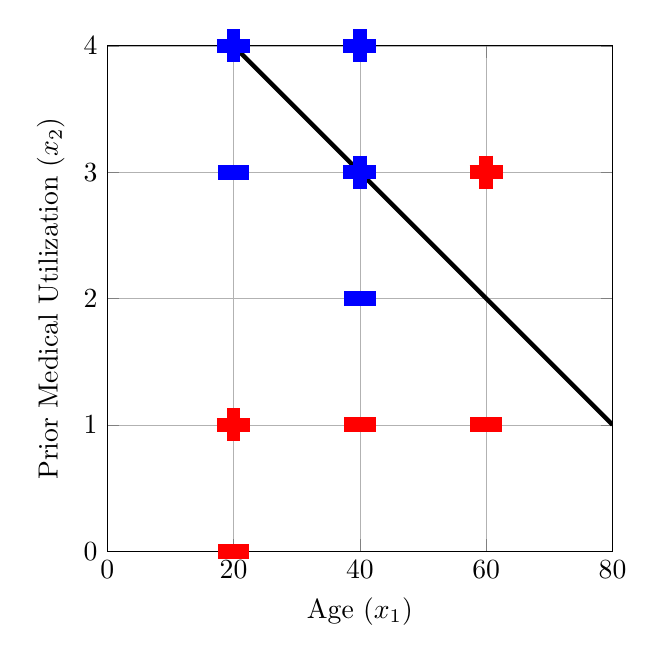
\begin{tikzpicture}
    \begin{axis}[
        width=8cm,
        height=8cm,
        axis equal,
        xmin=0, xmax=80,
        ymin=0, ymax=4,
        xlabel={$\text{Age } (x_1)$},
        ylabel={$\text{Prior Medical Utilization } (x_2)$},
        xtick={0,20,40,60,80},
        ytick={0,1,2,3,4}, 
        x=2cm/20,
        y=2cm,
        grid=both,
        grid style={line width=.1pt, draw=gray!30}, 
        major grid style={line width=.2pt,draw=gray!60},
        minor tick num=0 
    ]
    
    \addplot[only marks, mark=+, mark size=6pt, mark options={blue, line width=5pt}] coordinates {
        (20,4) (40,4) (40,3)
    };
    
    \addplot[only marks, mark=+, mark size=6pt, mark options={red, line width=5pt}] coordinates {
        (20,1) (60,3)
    };
    
    \addplot[only marks, mark=square*, mark options={xscale=2.5, yscale=1, blue, line width=1.5pt}] coordinates {
        (20,3) (40,2)
    }; 
    
    \addplot[only marks, mark=square*, mark options={xscale=2.5, yscale=1, red, line width=1.5pt}] coordinates {
        (20,0) (40,1) (60,1)
    }; 
    
    \addplot[domain=0:80, black, ultra thick, samples=100] {x/-20 + 5};
    
    \end{axis}
    \end{tikzpicture}
    \end{center}
    What are the coordinates of the data point whose label would be flipped first by this pre-processing method?

    \begin{your_solution}[width = 4cm,height=2cm]
    %YOUR ANSWER
    \end{your_solution}
    

    \subpart[2] After flipping the label of the point you identified in the previous question, plot the linear separator with the highest accuracy. For your convenience, we have provided a mechanism for you to input your answer by specifying the coordinates of two points on the decision boundary. \\ 
    \textbf{Note:} Look at the LaTeX comments for instructions on how to redraw the decision boundry.

    %YOUR ANSWER (Change the following 4 values to specify the slope of the line)
    \def\xone{40}   % Change me! Coordinate 1 x_1 value
    \def\yone{3}    % Change me! Coordinate 1 x_2 value
    \def\xtwo{20}   % Change me! Coordinate 2 x_1 value
    \def\ytwo{4}    % Change me! Coordinate 1 x_2 value
    
    \pgfmathsetmacro{\slope}{(\ytwo - \yone) / (\xtwo - \xone)}
    \pgfmathsetmacro{\intercept}{\yone - \slope * \xone}
    
    \begin{center}
    \begin{tikzpicture}
    \begin{axis}[
        width=8cm,
        height=8cm,
        axis equal,
        xmin=0, xmax=80,
        ymin=0, ymax=4,
        xlabel={$\text{Age } (x_1)$},
        ylabel={$\text{Prior Medical Utilization } (x_2)$},
        xtick={0,20,40,60,80},
        ytick={0,1,2,3,4}, 
        x=2cm/20,
        y=2cm,
        grid=both,
        grid style={line width=.1pt, draw=gray!30}, 
        major grid style={line width=.2pt,draw=gray!60},
        minor tick num=0 
    ]
    
    \addplot[only marks, mark=+, mark size=6pt, mark options={blue, line width=5pt}] coordinates {
        (20,4) (40,4) (40,3)
    };
    
    \addplot[only marks, mark=+, mark size=6pt, mark options={red, line width=5pt}] coordinates {
        (20,1) (60,3)
    };
    
    \addplot[only marks, mark=square*, mark options={xscale=2.5, yscale=1, blue, line width=1.5pt}] coordinates {
        (20,3) (40,2)
    }; 
    
    \addplot[only marks, mark=square*, mark options={xscale=2.5, yscale=1, red, line width=1.5pt}] coordinates {
        (20,0) (40,1) (60,1)
    }; 
    
    \addplot[domain=0:80, black, ultra thick, samples=100] {\slope*x + \intercept};
    
    \end{axis}
    \end{tikzpicture}
    \end{center}

    
    \subpart[1] Using the linear decision boundary your plotted in the previous question, what are the coordinates of the data point whose label would be flipped next by this pre-processing method?
    
    \begin{your_solution}[width = 4cm,height=2cm]
    %YOUR ANSWER
    \end{your_solution}


    \subpart[1] \textbf{True or False:} The algorithm terminates at this point.
    \begin{checkboxes}
        \choice True 
        \choice False
    \end{checkboxes}
    
\end{subparts}


\part \textbf{The fairness impossibility theorem:} Prove by contradiction that if prevalence rate, $r_s = P[Y=1 | S = s]$ across the two groups $s \in \{\text{blue}, \text{red}\}$ is different, then there does not exists a classifier that can satisfy PPV parity, FPR parity, and FNR parity simultaneously.

\begin{subparts}
    \subpart[4] Verify that the following identify holds for any $s \in \{\text{blue}, \text{red}\}$:
    $$FPR_s = \frac{r_s}{1-r_s} \times (1-FNR_s) \times \frac{(1-PPV_s)}{PPV_s}$$.

    \begin{your_solution}[width = \linewidth,height=10cm]
    %YOUR ANSWER
    \end{your_solution}

    \subpart[4] Show that the expression from part (a) can be rewritten as $$1/r_s =1 + \frac{(1-FNR_s)}{FPR_s} \times \frac{(1-PPV_s)}{PPV_s} $$

    \begin{your_solution}[width = \linewidth,height=10cm]
    %YOUR ANSWER
    \end{your_solution}
    \newpage
    \subpart[4] Finally, using results from parts (a) and (b), show that if $FPR_s, FNR_s,$ and $PPV_s$ are equal for $s \in \{\text{blue}, \text{red}\}$, then $r_s$ must be equal for $s \in \{\text{blue}, \text{red}\}$, which is a contradiction.

    \begin{your_solution}[width = \linewidth,height=10cm]
    %YOUR ANSWER
    \end{your_solution}
\end{subparts}


\end{parts} 
\newpage
\section{Collaboration Questions}
After you have completed all other components of this assignment, report your answers to these questions regarding the collaboration policy. Details of the policy can be found \href{http://www.cs.cmu.edu/~mgormley/courses/10601/syllabus.html}{here}.
\begin{enumerate}
    \item Did you receive any help whatsoever from anyone in solving this assignment? If so, include full details.
    \item Did you give any help whatsoever to anyone in solving this assignment? If so, include full details.
    \item Did you find or come across code that implements any part of this assignment? If so, include full details.
\end{enumerate}

\begin{your_solution}[height=6cm]
% YOUR ANSWER 

\end{your_solution}
\end{questions}


\end{document}